\section{Parameter correlation}\label{sec:parametercorrelation}

	The Fisher's information matrix for a maximum likelihood problem described by a multivariate normally distributed statistical model is defined to be the negative of the second partial derivatives of the log-likelihood function with respect to the parameters, $\xi_i$, evaluated at the maximum likelihood estimates. When converting to least squares minimization, which is equivalent of a negative log-likelihood minimization, the information matrix is defined to be
%==========================================================%
%-------------------	begin EQUATION 	-------------------%
\begin{equation}\label{eqn:informationmatrix}
\begin{aligned}
\mathcal{I}_{jk} = \dmd{\mathcal{F}}{2}{\xi_j}{}{\xi_k}{} = \mathcal{H}_{jk},
\end{aligned}
\end{equation}
%-------------------	 end EQUATION 	-------------------%
%==========================================================%
which is also exactly the Hessian matrix, $\mathbfcal{H}$, at the best fit value. The D-optimality is the determinant of this information matrix, whereas other optimality measures are mostly similar functions of this information matrix. The main reason is because, for a maximum likelihood problem governed by a normally distributed statistical model, the covariance matrix is exactly proportional to the inverse of the information matrix,
%==========================================================%
%-------------------	begin EQUATION 	-------------------%
\begin{equation}\label{eqn:covariancematrix}
\begin{aligned}
\mathbf{Cov} = \sigma^2 \mathbfcal{I}^{-1},
\end{aligned}
\end{equation}
%-------------------	 end EQUATION 	-------------------%
%==========================================================%
where $\sigma^2$ is the scalar variance of the statistical model, and can be estimated by the mean squared error weighted by the degree of freedom. Maximizing the D-optimality is equivalent of minimizing the variance of each parameter along with minimizing the covariance between parameters. Defining the objective function as
%==========================================================%
%-------------------	begin EQUATION 	-------------------%
\begin{equation}
\begin{aligned}
\mathcal{F} = \sum_i \left(f(x_i) - f_i\right)^2,
\end{aligned}
\end{equation}
%-------------------	 end EQUATION 	-------------------%
%----------------------------------------------------------%
where $f(x_i)$ is the model and $f_i$ are date points, the information matrix, or Hessian matrix, is given by 
%==========================================================%
%-------------------	begin EQUATION 	-------------------%
\begin{equation}\label{eqn:hessianmatrix}
\begin{aligned}
\dpd{\mathcal{F}}{\xi_j} =& \sum_i 2\left(f(x_i) - f_i\right)\dpd{f(x_i)}{\xi_j}	\\
\mathcal{H}_{jk} = \dmd{\mathcal{F}}{2}{\xi_j}{}{\xi_k}{} =& \sum_i 2\dpd{f(x_i)}{\xi_k}\dpd{f(x_i)}{\xi_j}	+ 2\left(f(x_i) - f_i\right)\dmd{f(x_i)}{2}{\xi_j}{}{\xi_k}{}
\end{aligned}
\end{equation}
%-------------------	 end EQUATION 	-------------------%
%----------------------------------------------------------%
Note here that $\mathcal{J}_{ij} = \dpd{f(x_i)}{\xi_j}$ is the Jacobian matrix for the non-linear least squares problem, and when the errors are small, i.e. when the model fits the data, in other words such that $\left(f(x_i) - f_i\right)$ is small or approximately 0, then the information matrix can by approximated by  
\begin{equation}
\mathcal{I}_{jk} \approx \mathcal{J}_{ji}\mathcal{J}_{ik} \quad \mathrm{or} \quad
\mathbfcal{I} \approx \mathbfcal{J}^\mathsf{T}\mathbfcal{J},
\end{equation}
a form much more familiar to most doing nonlinear least squares parameter estimation. 


	For $\Psi_{eff}$ (Eqn. \ref{eqn:finalexponentialmodelformscaled}), let $f = c_0Q^\prime e^{Q}$ be the stress, where $Q^\prime$ is one of $\pd{Q}{E_m}$, $\pd{Q}{E_n}$, or $\pd{Q}{E_\phi}$. The Jacobian matrix is thus, 
\begin{equation}	
\mathcal{J}_{ij} = Q^\prime e^Q \delta_{0j} + c_0 e^Q \dpd{Q^\prime}{\xi_j}+ c_0Q^\prime e^Q \dpd{Q}{\xi_j}
\end{equation}
Note that since $Q$ is a sum of polynomials, the second partial derivatives of $Q$ and $Q^\prime$ with respect to $\mathbf{\xi}$ is precisely 0,
\begin{equation}		
\md{Q}{2}{\xi_j}{}{\xi_k}{}  = \md{Q^\prime}{2}{\xi_j}{}{\xi_k}{} = 0.
\end{equation}
Thus,
\begin{equation}	
\begin{aligned}
\dmd{f}{2}{\xi_j}{}{\xi_k}{} =& e^Q \delta_{0j}\dpd{Q^\prime}{\xi_k} + Q^\prime e^Q \delta_{0j}\dpd{Q}{\xi_k} 
+  e^Q\dpd{Q^\prime}{\xi_j}\delta_{0k} + c_0 e^Q\dpd{Q^\prime}{\xi_j}\dpd{Q}{\xi_k} 
+ Q^\prime e^Q \dpd{Q}{\xi_j}\delta_{0k} 	\\
&+ c_0e^Q \dpd{Q}{\xi_j}\dpd{Q^\prime}{\xi_k}
+ c_0Q^\prime e^Q \dpd{Q}{\xi_j}\dpd{Q}{\xi_k} 
\end{aligned}
\end{equation}
and the Hessian matrix is given by
% \begin{equation}	
% \begin{aligned}
% \mathcal{H}_{jk} &= 2\sum_i\left[ (Q^\prime e^Q)^2  \delta_{0j}\delta_{0k} + c_0Q^\prime e^{2Q} \delta_{0j}\dpd{Q^\prime}{\xi_k}+ c_0 (Q^\prime e^Q)^2 \delta_{0j}\dpd{Q}{\xi_k}\right.	\\
% &+c_0Q^\prime e^{2Q} \dpd{Q^\prime}{\xi_j} \delta_{0k} + (c_0 e^Q)^2 \dpd{Q^\prime}{\xi_j}\dpd{Q^\prime}{\xi_k}+ (c_0e^Q)^2Q^\prime  \dpd{Q^\prime}{\xi_j}\dpd{Q}{\xi_k}	\\
% &+ c_0(Q^\prime e^Q)^2 \dpd{Q}{\xi_j}\delta_{0k} + Q^\prime (c_0 e^Q)^2 \dpd{Q}{\xi_j}\dpd{Q^\prime}{\xi_k}+ (c_0Q^\prime e^Q)^2 \dpd{Q}{\xi_j}\dpd{Q}{\xi_k}	\\
% &+ (c_0Q^\prime e^Q - f_i)\left( e^Q \delta_{0j}\dpd{Q^\prime}{\xi_k} + Q^\prime e^Q \delta_{0j}\dpd{Q}{\xi_k} 
% +  e^Q\dpd{Q^\prime}{\xi_j}\delta_{0k} 
% \right.	\\
% &\left.\left.+ c_0 e^Q\dpd{Q^\prime}{\xi_j}\dpd{Q}{\xi_k} + Q^\prime e^Q \dpd{Q}{\xi_j}\delta_{0k}  + c_0e^Q \dpd{Q}{\xi_j}\dpd{Q^\prime}{\xi_k}
% + c_0Q^\prime e^Q \dpd{Q}{\xi_j}\dpd{Q}{\xi_k} \right)\right]
% \end{aligned}
% \end{equation}

\begin{equation}	
\begin{aligned}
\mathcal{H}_{jk} &= 2\sum_i\left[ (Q^\prime e^Q)^2  \delta_{0j}\delta_{0k} + c_0Q^\prime e^{2Q} \left(\delta_{0j}\dpd{Q^\prime}{\xi_k} + \dpd{Q^\prime}{\xi_j} \delta_{0k}\right) + c_0 (Q^\prime e^Q)^2 \left(\delta_{0j}\dpd{Q}{\xi_k} + \dpd{Q}{\xi_j}\delta_{0k}\right)   \right.	\\
&+ (c_0 e^Q)^2 \dpd{Q^\prime}{\xi_j}\dpd{Q^\prime}{\xi_k} +  (c_0e^Q)^2Q^\prime \left( \dpd{Q^\prime}{\xi_j}\dpd{Q}{\xi_k}	+ \dpd{Q}{\xi_j}\dpd{Q^\prime}{\xi_k}\right) + (c_0Q^\prime e^Q)^2 \dpd{Q}{\xi_j}\dpd{Q}{\xi_k}	\\
&+ (c_0Q^\prime e^Q - f_i)\left.\left[ e^Q \left(\delta_{0j}\dpd{Q^\prime}{\xi_k} + \dpd{Q^\prime}{\xi_j}\delta_{0k}\right) + Q^\prime e^Q \left(\delta_{0j}\dpd{Q}{\xi_k}  + \dpd{Q}{\xi_j}\delta_{0k}\right)
\right.\right.	\\
&\left.\left.+ c_0 e^Q\left(\dpd{Q^\prime}{\xi_j}\dpd{Q}{\xi_k}  +  \dpd{Q}{\xi_j}\dpd{Q^\prime}{\xi_k}\right)
+ c_0Q^\prime e^Q \dpd{Q}{\xi_j}\dpd{Q}{\xi_k} \right]\right].
\end{aligned}
\end{equation}
Here, the summation is over each data point $i$ and then sums for each component of stress $S_m$, $S_n$, and $S_\phi$ for $Q^\prime = \pd{Q}{E_m}$, $\pd{Q}{E_n}$ and $\pd{Q}{E_\phi}$ respectively. 

	Using this approach, we compared the covariance of the model parameters for with Green-Lagrange strains and with Hencky strains for the Fung model (Table \ref{tb:correlationE}\&\ref{tb:correlationG}, Fig. \ref{fig:gvsecorrelation}), $\Psi_{eff}$ (Eqn. \ref{eqn:finalexponentialmodelformscaled}) (Fig. \ref{fig:gvsecorrelationeff}), and the polynomial series type model with $i,j,k \leq 6$ (Fig. \ref{fig:gvsecorrelationpoly}). The Hencky strains have lower parameter correlation as shown, but this appears to be minimal for $\Psi_{eff}$. The main benefits are seen with higher order coupling terms, and may still be beneficial for other constitutive models forms. 



%----------------------------------------------------------%
%-------------------	begin TABLE 	-------------------%
\begin{table}[ht]
\caption{The correlation between model parameter when using Green Lagrange strains}
\begin{center}
\label{tb:correlationE}
\small 
\begin{tabular}{|l|cccccc|}
\hline
		 & $b_1$ & $b_2$& $b_3$& $b_4$& $b_5$& $b_6$ \\
\hline  
$b_1$	 & 1. & 0.0439916 & 0.0195981 & -0.571707 & -0.545413 & 0.314503 \\
$b_2$	 & 0.0439916 & 1. & 0.0195981 & -0.571707 & 0.314503 & -0.545413 \\
$b_3$	 & 0.0195981 & 0.0195981 & 1. & 0.306268 & -0.555437 & -0.555437 \\
$b_4$	 & -0.571707 & -0.571707 & 0.306268 & 1. & -0.167068 & -0.167068 \\
$b_5$	 & -0.545413 & 0.314503 & -0.555437 & -0.167068 & 1. & -0.179471 \\
$b_6$	 & 0.314503 & -0.545413 & -0.555437 & -0.167068 & -0.179471 & 1. \\
\hline
\end{tabular}
\normalsize
\end{center}
\end{table}
%-------------------	 end TABLE 		-------------------%
%----------------------------------------------------------%


%----------------------------------------------------------%
%-------------------	begin TABLE 	-------------------%
\begin{table}[ht]
\caption{The correlation between model parameter when using Hencky strains}
\begin{center}
\label{tb:correlationG}
\small
\begin{tabular}{|l|cccccc|}
\hline
		& $b_1$ & $b_2$& $b_3$& $b_4$& $b_5$& $b_6$ \\
\hline
$b_1$	& 1. & 0.0709169 & 0.016636 & -0.590101 & -0.576084 & 0.322457 \\
$b_2$	& 0.0709169 & 1. & -0.0173651 & -0.601126 & 0.282699 & -0.49857 \\
$b_3$	& 0.016636 & -0.0173651 & 1. & 0.294546 & -0.514879 & -0.524943 \\
$b_4$	& -0.590101 & -0.601126 & 0.294546 & 1. & -0.100413 & -0.171661 \\
$b_5$	& -0.576084 & 0.282699 & -0.514879 & -0.100413 & 1. & -0.222942 \\
$b_6$	& 0.322457 & -0.49857 & -0.524943 & -0.171661 & -0.222942 & 1. \\
\hline
\end{tabular}
\normalsize
\end{center}
\end{table}
%-------------------	 end TABLE 		-------------------%
%----------------------------------------------------------%


%%%%%%%%%%%%%%%%%%%%%%%%%%%%%%%%%%%%%%%%%%%%%%%%%%%%%%%%%%%%
%-------------------	begin FIGURE 	-------------------%
\begin{figure}
\centering
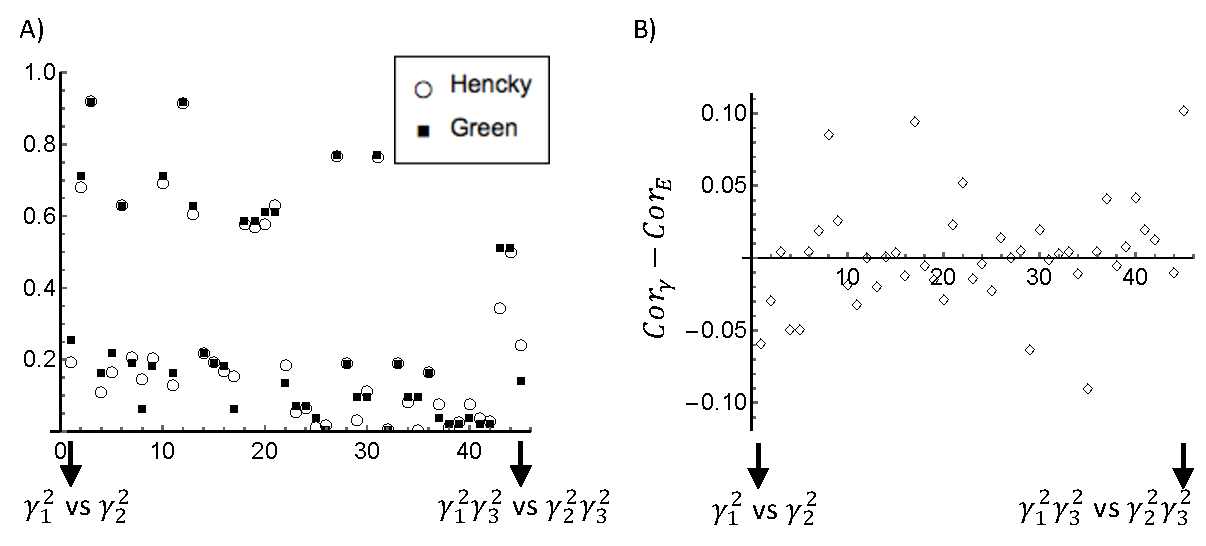
\includegraphics[width=6.0in]{Figures/gvsecorrelationeff}
\caption{(A) The correlation between parameters pairs in $\Psi_{eff}$ (Eqn. \ref{eqn:finalexponentialmodelformscaled}) when using Green-Lagrange vs Hencky strains. (B) The difference in correlation between each pair of parameters is minimal.}
\label{fig:gvsecorrelationeff}
\end{figure}
%-------------------	 end FIGURE 	-------------------%
%%%%%%%%%%%%%%%%%%%%%%%%%%%%%%%%%%%%%%%%%%%%%%%%%%%%%%%%%%%%


%%%%%%%%%%%%%%%%%%%%%%%%%%%%%%%%%%%%%%%%%%%%%%%%%%%%%%%%%%%%
%-------------------	begin FIGURE 	-------------------%
\begin{figure}
\centering
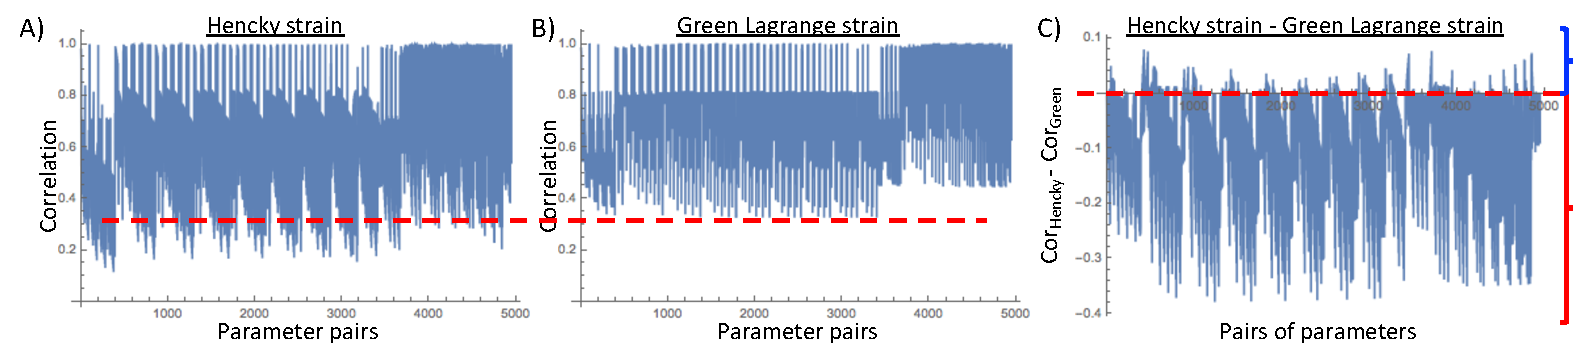
\includegraphics[width=6.5in]{Figures/gvsecorrelationpoly}
\caption{(A) The correlation between parameters pairs in a polynomial series type model with powers up to 6 when using Green-Lagrange vs (B) Hencky strains. (C) The difference in correlation between each pair of parameters. The red bracketed terms are benefited from using Hencky strains whereas the significantly fewer blue bracketed terms has better correlations with Green-Lagrange strain.}
\label{fig:gvsecorrelationpoly}
\end{figure}
%-------------------	 end FIGURE 	-------------------%
%%%%%%%%%%%%%%%%%%%%%%%%%%%%%%%%%%%%%%%%%%%%%%%%%%%%%%%%%%%%














